\begin{figure}[!h]
    \centering
    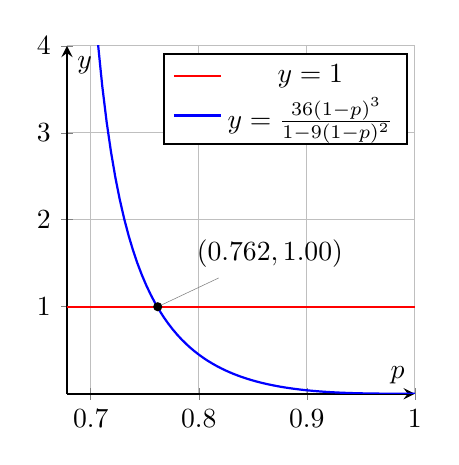
\begin{tikzpicture}
    \begin{axis}
    [xlabel={$p$}, 
     ylabel={$y$},
     axis lines=middle,
     grid,
     thick,
     domain=0.678:1,
     width=6cm,
     height=6cm,
     samples=80,
     ymin=0,
     ymax=4,
     %legend pos=outer north east
    ]
    \addplot+[no marks, red] {1};
    \addlegendentry{$y = 1$}
    \addplot+[no marks, blue] {(36 * (1-x)^3) / (1 - 9*(1-x)^2)};
    \addlegendentry{$y = \frac{36(1-p)^3}{1 - 9(1 - p)^2}$}
    \node[circle, fill=black, scale=0.35, pin=45:{$(0.762, 1.00)$}] at (axis cs:0.762, 1.0) {};
    \end{axis}
    \end{tikzpicture}
    \caption{The upper bound on $\Pp(\abs{C} < \infty)$}
    \label{fig:pc_upper_bound_plot}
\end{figure}